\title{Resumen de fisica 1}

\author{Mateo P. Cetti}

\documentclass[10pt]{article}

\usepackage{amsmath}
\usepackage{amsfonts}
\usepackage{graphicx}

\begin{document} 
\maketitle

\section{Óptica - Luz}

\paragraph{Naturaleza de la luz}

Se debe considerar que la luz tiene \textbf{doble naturaleza} en algunos casos exhibe características de una \textbf{onda} y en otras de una \textbf{partícula} (onda electromagnetica sinusoidal o rayo de luz)\\
\linebreak
El modelo de cuantización supone que la \textbf{energía} de una onda luminosa está presente en partículas llamadas \textbf{fotones}; por tanto, se dice que la energía está \textbf{cuantizada}. La energía de un fotón es proporcional a la frecuencia de la onda electromagnética. $E = hf \rightarrow h = 6.63 \times 10^{-34} J\cdot s$ donde $h$ es la \textbf{constante de Plank}.\\

\paragraph{Mediciones de la rapidez de la luz}
Hubo muchos intentos de medir la rapidez de la luz. \textbf{Galilei} intento pero no pudo.\\ 
\textbf{Roemer} hizo la primera estimacion exitosa de la rapidez de la luz (Metodo astronomico de jupiter)\\
\textbf{Fizeau} Fue el primero en dar una estimacion de la velocidad de la luz con metodos terrestres. (Metodo del espejo y la rueda dentada).
\paragraph{Aproximación de un rayo en óptica geométrica}

En la \textbf{optica geometrica} la luz es entendida como un \textbf{rayo} que cambia de direccion cuando se encuentra con la superficie de un medio distinto.\\
\linebreak
En óptica geométrica se usa la aproximación de rayo, en donde una onda viaja a través de un medio uniforme en líneas rectas
en la dirección de los rayos.

\paragraph{La onda bajo reflexión}

Las ondas de luz reflejadas pueden estar en \textbf{direcciones distintas} de la dirección de las ondas incidentes (A diferencia de las ondas en cuerdas). Una reflexion es \textbf{especular} cuando se refleja desde una superficie \textbf{lisa}. En cambio es \textbf{difusa} cuando se refleja desde una superficie \textbf{rugosa}.\\
\linebreak
Considere un rayo de luz que viaja en el aire y que incide a un ángulo en una superficie plana y lisa. Los rayos incidente y reflejado forman ángulos $\theta_1$ y $\theta_1'$, respectivamente, donde los ángulos se observan entre la normal y los rayos.  Experimentos y teoría muestran que el \textbf{ángulo de reflexión es igual al ángulo de incidencia} $\theta_1 = \theta_1'$ (\textbf{Ley de reflexion})

\paragraph{La onda bajo refracción}

Cuando un rayo de luz que se mueve por un medio transparente encuentra una frontera que lleva a otro medio de igual característica, parte de la energía se \textbf{refleja} y parte penetra al segundo medio (se \textbf{refracta}).\\
\linebreak
\textbf{Angulo de refraccion: } $\dfrac{sen \theta_2}{sen \theta_1} = \dfrac{v_1}{v_2}$\\
\linebreak
La trayectoria de un rayo de luz que pasa por una superficie refractaria es \textbf{reversible}. \\
\linebreak
Cuando la luz se mueve de un material en el que su \textbf{rapidez es alta} a un material en el que su \textbf{rapidez es menor}, el ángulo de refracción $\theta_2$ es \textbf{menor} que el ángulo de incidencia $\theta_1$, y el rayo se dobla hacia la normal. Si el rayo se mueve de un material en el que la luz se mueve con \textbf{más lentitud} hacia un material en el que se mueve con \textbf{más rapidez}, $\theta_2$ es \textbf{mayor} que $\theta_1$ y el rayo se dobla alejándose de la normal.

\paragraph{Índice de refracción}

La \textbf{rapidez de la luz} en cualquier material es \textbf{menor que en el vacío}. De hecho, la luz se desplaza a su máxima rapidez en el vacío. Es conveniente definir el \textbf{índice de refracción} $n$ de un medio como la relación $n = \dfrac{\text{rapidez de la luz en el vacio}}{\text{rapidez de la luz en el medio}} = \dfrac{c}{v}$\\
\linebreak
Cuando la luz pasa de un medio a otro, su \textbf{frecuencia} no cambia, pero sí lo hace su \textbf{longitud de onda}\\
\linebreak
\textbf{Ley de refraccion de Snell}
\begin{equation*}
	n_1 \cdot sen \theta_1 = n_2 \cdot sen \theta_2
\end{equation*}

\paragraph{Reflexión interna total}

Se presenta al dirigir luz desde un medio con un índice de refracción determinado \textbf{hacia otro} que tenga un índice de refracción \textbf{menor}. En algún ángulo particular de incidencia $\theta_c$ , denominado \textbf{ángulo crítico}, el rayo de luz refractado se mueve \textbf{paralelo} a la frontera, de modo que $\theta_2 = 90°$. Para ángulos de incidencia \textbf{mayores} a $\theta_c$, el rayo se refleja \textbf{por completo} en la frontera

\begin{equation*}
	sen \theta_c = \frac{n_2}{n_1} \rightarrow n_1 > n_2
\end{equation*}

Repetimos: \textbf{, la reflexión interna total se presenta sólo cuando la luz se dirige de un medio de índice de refracción conocido hacia un medio de índice de refracción menor.}\\
\linebreak
El ángulo crítico para la reflexión interna total es \textbf{pequeño} cuando $n_1$ es considerablemente \textbf{mayor} a $n_2$.

\section{Formación de imágenes}

\paragraph{Imágenes formadas por espejos planos}

Imagine una fuente puntual de luz colocada en $O$ a una distancia $p$ (\textbf{distancia objeto}) frente a un espejo plano. Después de reflejarse, los rayos siguen un proceso de divergencia (extensiones de los rayos divergentes hacia atrás,
hasta un punto de intersección en $I$).  Para el observador parece que los rayos divergentes surgen del punto $I$ detrás del espejo. El punto I, que está a una distancia $q$ (\textbf{distancia de imagen}) detrás del espejo, se conoce como \textbf{imagen} del objeto en $O$.  Las imágenes están localizadas ya sea en un punto a partir del cual los rayos luminosos realmente divergen o en un punto a partir del cual parece que divergen. (?)\\
\linebreak
Las imágenes se clasifican en \textbf{reales} o \textbf{virtuales}. Una imagen real es la que se forma cuando los rayos luminosos \textbf{pasan a través y divergen del punto de imagen}; una imagen virtual es la que se forma cuando los rayos luminosos \textbf{no pasan a través del punto} de imagen sino que sólo parecen divergir de dicho punto. La imagen de un objeto vista en un espejo plano \textbf{es siempre virtual}.  la imagen formada por un objeto colocado frente a un espejo plano \textbf{está tan lejos} detrás del espejo \textbf{como lo está el objeto} frente a él. Tambien,  la altura del objeto $h$ es igual a la altura de la imagen $h'$ (\textbf{Aumento lateral}) $M = \dfrac{h'}{h}$

\paragraph{Imágenes formadas por espejos esféricos}

\paragraph{Espejos cóncavos}  Estos espejos tienen \textbf{radio de curvatura} $R$, y su \textbf{centro de curvatura} es el punto $C$.\\
Ahora considere una fuente de luz puntual colocada en el punto $O$, a la izquierda de $C$. En la figura se muestran \textbf{dos rayos divergentes} que se \textbf{originan en $O$}. Después de reflejarse en el espejo, estos rayos \textbf{convergen} y se cruzan \textbf{en la imagen} que aparece en el punto $I$. Después continúan divergiendo alejándose de I como si en ese punto existiera un objeto. Como resultado, \textbf{la imagen en el punto $I$ es real}. Despues de una demostracion re loca tenemos que:\\
\linebreak
El \textbf{Aumento de la imagen} es:
\begin{equation*}
	M = \dfrac{-q}{p}
\end{equation*}

y la \textbf{ecuacion del espejo segun el radio de curvatura}
\begin{equation*}
	\dfrac{1}{p} + \dfrac{1}{q} = \dfrac{2}{R}
\end{equation*}

cuando el objeto está muy lejos del espejo, el punto imagen está a la \textbf{mitad del camino} entre el centro de curvatura y el punto central sobre el espejo. Los rayos incidentes del objeto son esencialmente paralelos en estafi gura porque se supone que la fuente está muy lejos del espejo. En este caso en especial, se le llama al punto de imagen \textbf{foco F} y a la distancia de imagen \textbf{distancia focal $f$}, donde: 

\begin{equation*}
 f = \dfrac{R}{2}
\end{equation*}
Ecuacion del espejo en funcion de la distancia focal:
\begin{equation*}
	\dfrac{1}{p} + \dfrac{1}{q} = \dfrac{1}{f}
\end{equation*}

\paragraph{Espejos convexos}
los rayos de cualquier punto de un objeto \textbf{divergen} después de haberse reflejado, como si vinieran de algún punto de detrás del espejo (la imagen es \textbf{virtual}). Ademas, la imagen siempre es \textbf{vertical} y es \textbf{menor} que el objeto.\\

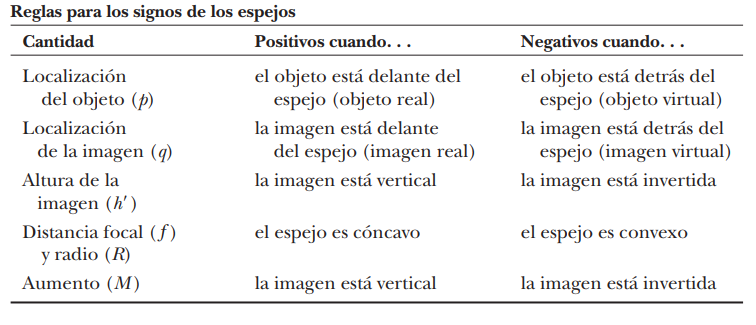
\includegraphics[width = 350px]{tabla_espejos.png}

\paragraph{Diagramas de rayos para espejos}
Para dibujar el diagrama de un rayo, es necesario conocer la posición del objeto y la localización del foco, así como el centro de curvatura del espejo. Después, dibuje tres rayos principales para localizar la imagen.\\
En el caso de espejos cóncavos, trace los tres rayos principales siguientes
\begin{itemize}
	\item El rayo 1, desde la parte superior del objeto, en paralelo al eje principal, y se refleja a través del foco F
	\item El rayo 2, desde la parte superior del objeto a través del foco (o como si viniera del foco si $p < f$ ) y se refleja paralelo al eje principal.
	\item El rayo 3, desde la parte superior del objeto a través del centro de curvatura C y se refleja de regreso sobre sí mismo.
\end{itemize}
En el caso de los espejos convexos, trace los tres rayos principales siguientes:
\begin{itemize}
	\item El rayo 1 se dibuja desde la parte superior del objeto paralelo al eje principal y se refleja alejándose del foco F.
	\item El rayo 2 El rayo 2, se dibuja desde la parte superior del objeto hacia el foco en la cara posterior del espejo y se refleja paralelo al eje principal.
	\item El rayo 3 se dibuja desde la parte superior del objeto hacia el centro de curvatura C en la cara posterior del espejo y se refleja de regreso sobre sí mismo.
\end{itemize}
\paragraph{Imágenes formadas por refracción}
Considere dos medios transparentes con índices de refracción $n_1$ y $n_2$, donde los límites entre los dos medios forman una superficie esférica de radio $R$. Suponga que el objeto en $O$ está en el medio cuyo índice de refracción es $n_1$. Consideremos los rayos paraxiales que salen de $O$. Como verá, todos estos rayos se refractan en la superficie esférica y se enfocan en un único punto $I$, el punto imagen.\\
Despues de una demostracion bien chingona, se llega a la \textbf{relación entre distancia objeto y distancia imagen para una superficie refractora}
\begin{equation*}
	\dfrac{n_1}{p} + \dfrac{n_2}{q} = \dfrac{n_2-n_1}{R}
\end{equation*}
Igual que en el caso de los espejos, es necesario utilizar una convención para los signos si desea aplicar esta ecuación a diferentes casos:

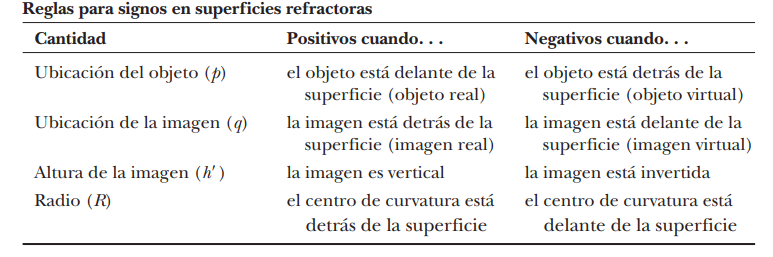
\includegraphics[width = 400px]{tabla_vidrios.png}

\paragraph{Superficies refractoras planas}

Si una superficie refractora es plana, en tal caso R es infinito y la ecuación se reduce a
\begin{equation*}
	q = - \dfrac{n_2}{n_1}p
\end{equation*}

La imagen formada por una superficie refractora plana está en el mismo lado de la superficie que el objeto (y es virtual).

\paragraph{Lentes delgadas}

La luz que pasa a través de ella experimenta una refracción en \textbf{dos superficies}. El desarrollo a seguir está en función de la creencia de que \textbf{la imagen formada por una superficie refractora sirve como el objeto para la segunda superficie}.\\
\linebreak
\textbf{Ecuacion de los fabricantes de lentes}
\begin{equation*}
	\dfrac{1}{f} = (n-1)\left( \dfrac{1}{R_1} - \dfrac{1}{R_2}  \right) 
\end{equation*}
\textbf{ ecuación de las lentes delgadas}
\begin{equation*}
	\dfrac{1}{p} + \dfrac{1}{q} = \dfrac{1}{f}
\end{equation*}
\textbf{Aumento de las imagenes}
\begin{equation*}
	M = -\dfrac{q}{p}
\end{equation*}

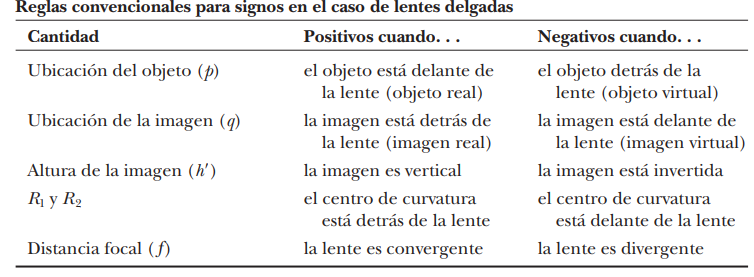
\includegraphics[width = 400px]{tabla_lentes.png}

\paragraph{Diagramas de rayos para lentes delgadas}
Esta parte me dio flojera copiar, aca va una screen :V

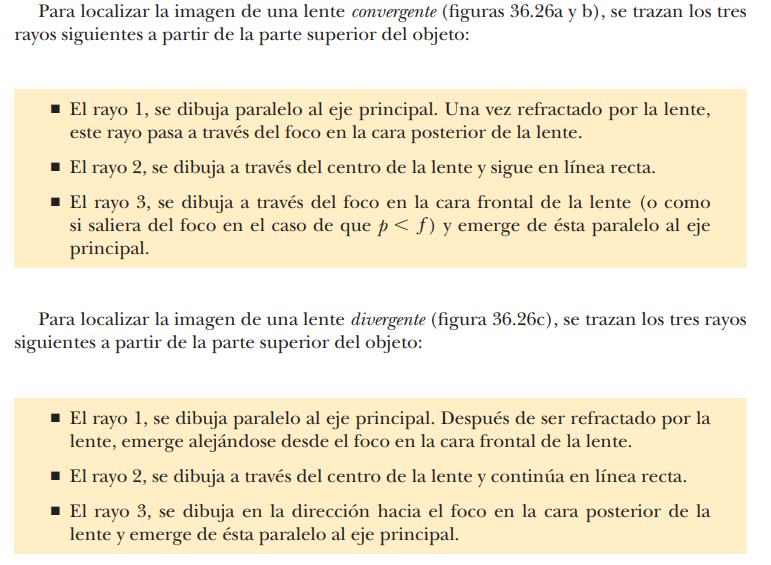
\includegraphics[width = 400px]{vagancia.png}

\paragraph{Combinación de lentes delgadas}

el aumento general de la imagen causada por la combinación de las lentes es el producto de los aumentos individuales. $M = M_1 M_2$\\
\linebreak
\textbf{Distancia focal para una combinación de dos lentes delgadas en contacto} $\dfrac{1}{f} = \dfrac{1}{f_1} + \dfrac{1}{f_2}$

\section{ Rotación de un objeto rígido en torno a un eje fijo}

el \textbf{movimiento} de un objeto extendido se analiza al representarlo como un \textbf{conjunto de partículas}, cada una con su \textbf{propia velocidad y aceleración} lineales. Un \textbf{objeto rígido} no es deformable; es decir, las \textbf{ubicaciones relativas} de todas las \textbf{partículas} de que está compuesto permanecen \textbf{constantes}.\\
\pagebreak

\paragraph{Posición, velocidad y aceleración angular}.

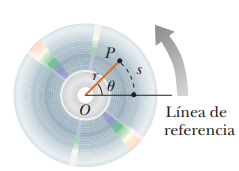
\includegraphics[width = 200px]{rotacion_1.png}

El disco da vueltas en torno a un \textbf{eje fijo} perpendicular al plano de la figura que pasa a través del centro del disco en $O$. Un pequeño elemento del disco modelado como \textbf{partícula} en $P$ está a una \textbf{distancia} fija $r$ desde el origen y gira en torno a él en un círculo de radio r.  A medida que la partícula se mueve a lo largo del círculo , se mueve a través de una \textbf{longitud de arco} $s$. La longitud de arco $s$ se relaciona con el ángulo $\theta$ mediante: 
\begin{equation*}
	s = r\theta
\end{equation*}
Como el objeto es \textbf{rigido},  se puede asociar el ángulo $\theta$ con \textbf{todo el objeto} rígido así como con una \textbf{partícula individual}, que permite definir la \textbf{posición angular} de un objeto rígido en su movimiento rotacional.\\
\linebreak
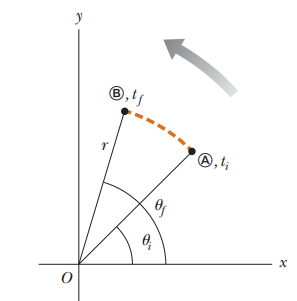
\includegraphics[width = 200px]{desplazamiento_angular.png}\\
\textbf{Desplazamiento angular: } $\Delta \theta = \theta_f - \theta_i$\\
\linebreak
\textbf{Rapidez angular} $w = \dfrac{d\theta}{dt}$\\
\linebreak
\textbf{Rapidez angular promedio} $w_{prom} = \dfrac{\Delta \theta}{\Delta t}$\\
\linebreak
\textbf{Aceleracion angular promedio} $w_{prom} = \dfrac{\Delta w}{\Delta t}$\\
\linebreak
\textbf{Aceleracion angular} $w = \dfrac{dw}{dt}$\\
\linebreak

\textbf{Cuando un objeto rígido en rotación respecto a un eje fijo, cada partícula sobre el objeto da vueltas a través del mismo ángulo en un intervalo de tiempo determinado y tiene la misma rapidez angular y la misma aceleración angular}

\paragraph{Cinemática rotacional: Objeto rígido bajo aceleración angular constante}.

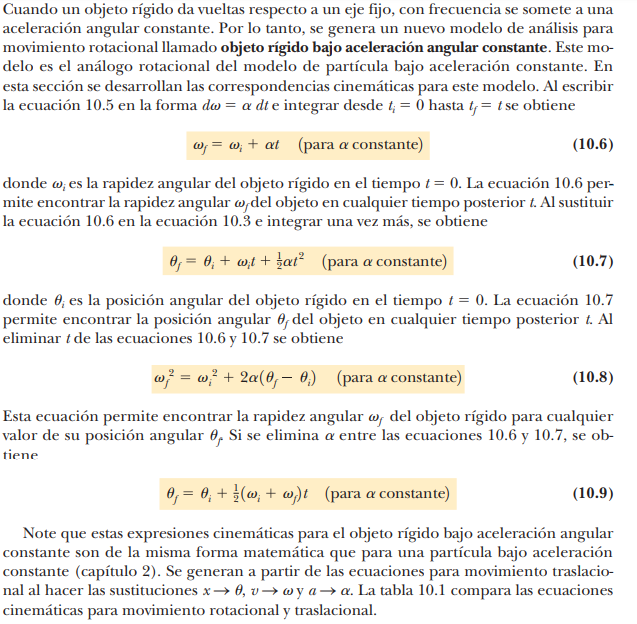
\includegraphics[width = 350px]{vagancia_2.png}\\

\paragraph{Cantidades angulares y traslacionales}

Se muestran algunas relaciones útiles entre la rapidez y la aceleración angulares de un objeto rígido en rotación y la rapidez y la aceleración traslacionales de un punto en el objeto. Importante tener en cuenta que  toda partícula del objeto se mueve
en un círculo cuyo centro está en el eje de rotación.\\
\linebreak
La rapidez tangencial de un punto sobre un objeto rígido en rotación es igual a la distancia perpendicular de dicho punto desde el eje de rotación, multiplicada por la rapidez angular. $v = rw$\\
\linebreak
la componente tangencial de la aceleración traslacional de un punto sobre un objeto rígido en rotación es igual a la distancia perpendicular del punto desde el eje de rotación, multiplicada por la aceleración angular. $a_t = r\alpha$\\
\linebreak
La aceleración centrípeta en dicho punto se puede expresar en términos de rapidez angular como $a_c = rw^2$

\paragraph{Energía cinética rotacional}
Las partículas individuales que conforman el objeto en rotación se mueven a través del espacio (en el movimiento rotacional hay energía cinética asociada).\\
\linebreak
\textbf{Momento de inercia} $I = \sum_i m_i r_i^2$\\
\linebreak
\textbf{Energía cinética rotacional}
\begin{equation*}
	K_R = \dfrac{1}{2}Iw^2
\end{equation*}

\paragraph{Cálculo de momentos de inercia}
Momento de inercia de un objeto rígido:
\begin{equation*}
	I = \int r^2 dm
\end{equation*}

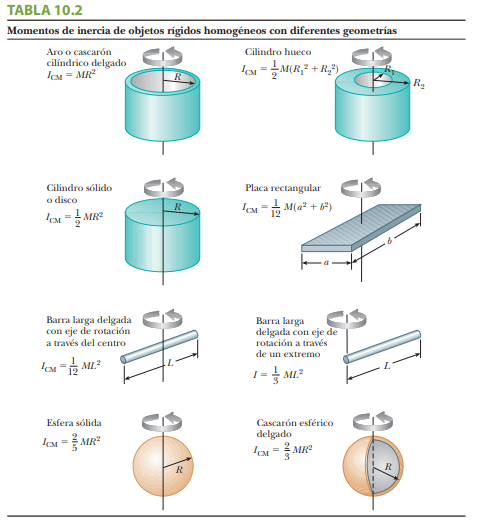
\includegraphics[width = 350px]{inercias.png}\\

El cálculo de momentos de inercia de un objeto en torno a un \textbf{eje arbitrario} puede ser
complicado, incluso para un objeto considerablemente simétrico. Por fortuna, el uso de
un importante teorema, llamado \textbf{teorema de ejes paralelos}, con frecuencia simplifica el
cálculo.

\begin{equation*}
	I = I_{CM} + MD^2
\end{equation*}

\paragraph{Momento de torsión}
Imagine que intenta dar vuelta una puerta y aplica una fuerza de magnitud F, perpendicular a la superficie de la puerta cerca de las bisagras y luego en diferentes distancias desde las bisagras. Usted logrará una relación de rotación más rápida para la puerta al aplicar la fuerza cerca de la perilla que al aplicarla cerca de las bisagras.\\
\linebreak
La tendencia de una fuerza a dar vuelta un objeto en torno a cierto eje se mide mediante una cantidad llamada momento de torsión $\overrightarrow{\tau}$

\begin{equation*}
	\tau rFsen\phi = Fd
\end{equation*}
donde $d$ es el \textbf{brazo de momento} ( distancia perpendicular desde el eje de rotación hasta la línea de acción)
\paragraph{Objeto rígido bajo un momento de torsión neto}
El momento de torsión neto que actúa sobre la partícula es proporcional a su
aceleración angular
\begin{equation*}
	\sum \tau = I\alpha
\end{equation*}

\paragraph{Consideraciones energéticas en el movimiento rotacional}

\textbf{ Potencia entregada a un objeto rígido en rotacion}
\begin{equation*}
	P = \dfrac{dW}{dt} = \tau w
\end{equation*}
\textbf{Teorema trabajo–energía cinética para movimiento rotacion}
\begin{equation*}
	\sum W = \frac{1}{2}Iw_f^2 - \frac{1}{2}Iw_i^2
\end{equation*}
Este teorema afirma que el trabajo neto invertido
por fuerzas externas en un objeto rígido simétrico en rotación en torno a un eje fijo es
igual al cambio en la energía rotacional del objeto
\paragraph{Movimiento de rodamiento de un objeto rígido}

la rapidez traslacional del centro de masa para movimiento de rodamiento puro
se conoce por $v_{CM} = Rw$ (R es radio)\\
 a magnitud de la aceleración lineal del centro de masa para movimiento de rodamiento puro es $a_{CM} = R\alpha$\\
\linebreak
Energía cinética total de un objeto en rodamiento
\begin{equation*}
	K = \frac{1}{2} I_{CM}w^2 + \frac{1}{2} Mv_{CM}^2
\end{equation*}
La energía cinética total de un objeto en rodamiento es la suma de la energía cinética rotacional en torno al centro de masa y la energía cinética traslacional del centro de masa.
\section{Cantidad de movimiento angular}

La cantidad de movimiento angular de un sistema se conserva si sobre el sistema no actúan momentos de torsión \textbf{externos}

\paragraph{Producto vectorial y momento de torsión}

El vector momento de torsión $\overrightarrow{\tau}$ se relaciona con los dos vectores $ \overrightarrow{r} \text{y} \overrightarrow{F}$. Es posible establecer una correspondencia matemática entre $\overrightarrow{\tau} \overrightarrow{r} \text{y} \overrightarrow{F}$ al usar una operación matemática llamada producto vectorial o producto cruz:

\begin{equation*}
	\overrightarrow{\tau} = \overrightarrow{r} \times \overrightarrow{F}
\end{equation*}

\paragraph{Cantidad de movimiento angular: el sistema no aislado}

La \textbf{cantidad de movimiento angular instantánea} $\overrightarrow{L}$ de una partícula en relación con un eje a través del origen $O$ se define mediante el producto cruz del vector de posición instantáneo de la partícula $\overrightarrow{r}$y su cantidad de movimiento lineal instantánea $\overrightarrow{p}$:
\begin{equation*}
	\overrightarrow{L} = \overrightarrow{r} \times \overrightarrow{p}
\end{equation*}
El momento de torsión que actúa sobre una partícula es igual a la relación de cambio en el tiempo de la cantidad de movimiento angular de la partícula. (Esto siempre y cuando se mida en torno al mismo eje)\\
\linebreak
\textbf{Importante:}  Si un sistema no es aislado en el sentido que existe un momento de torsión neto sobre él, el momento de torsión es igual a la rapidez de cambio en el tiempo de la cantidad de movimiento angular

\paragraph{Cantidad de movimiento angular de un objeto rígido giratorio}.

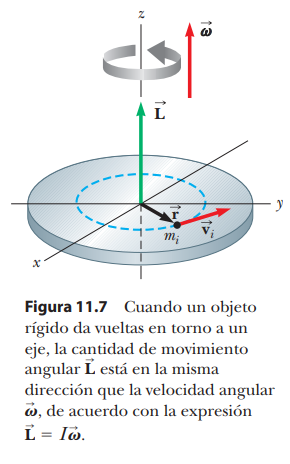
\includegraphics[width = 175px]{11.3.png}\\

El momento de torsión externo neto que actúa sobre un objeto rígido giratorio en torno a un eje fijo es igual al momento de inercia en torno al eje de rotación multiplicado por la aceleración angular del objeto en relación con dicho eje. (\textbf{Forma rotacional de la segunda ley de Newton})

\begin{equation*}
	\sum \tau_{ex} = I \alpha
\end{equation*}

\paragraph{El sistema aislado: conservación de cantidad de movimiento angular}.\\

\textbf{Conservación de cantidad de movimiento angular}La cantidad de movimiento angular total de un sistema es constante tanto en magnitud como en dirección si el momento de torsión externo neto que actúa sobre el sistema es cero, es decir, si el sistema está aislado. En este caso:

\begin{equation*}
	\overrightarrow{L}_{tot} = constante \textbf{ o } \overrightarrow{L}_i = \overrightarrow{L}_f 
\end{equation*}

un cambio en I para un sistema aislado requiere un cambio en v. En este caso, el principio de conservación de cantidad de movimiento angular se expresa como

\begin{equation*}
	I_i \omega_i = I_f \omega_f = \text{constante}
\end{equation*}
Esta expresión es válida tanto para rotación en torno a un eje fijo, como para rotación en torno a un eje a través del centro de masa de un sistema móvil en tanto dicho eje permanezca fijo en la dirección. Sólo se requiere que el momento de torsión externo neto sea cero.\\
\linebreak

Ahora se puede afirmar que la energía, la cantidad de movimiento lineal y la cantidad de movimiento angular de un sistema aislado se conservan.

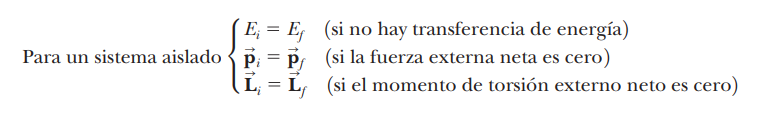
\includegraphics[width = 275px]{conservacion.png}\\

\section{Movimiento oscilatorio}

\paragraph{Movimiento de un objeto unido a un resorte}

Como un modelo de movimiento armónico simple considere un bloque de masa m unido al extremo de un resorte, con el bloque libre de moverse sobre una superficie horizontal sin fricción. Cuando el resorte no está estirado ni comprimido, el bloque
queda en reposo, en la posición llamada \textbf{posición de equilibrio} del sistema.\\
cuando el bloque se desplaza a una posición x, el resorte ejerce sobre el bloque una fuerza que es proporcional a la posición y se conoce por la \textbf{ley de Hooke}

\begin{equation*}
	F_s = -kx
\end{equation*}
Esta es laa \textbf{fuerza restauradora} porque siempre se dirige hacia la posición de equilibrio y, en consecuencia, es opuesta al desplazamiento del bloque desde el equilibrio.\\
\linebreak
La \textbf{aceleración} del bloque es proporcional a su \textbf{posición}, y la \textbf{dirección} de la aceleración es \textbf{opuesta} a la dirección del desplazamiento del bloque desde el equilibrio. Se dice que los sistemas que se comportan de esta forma exhiben \textbf{movimiento armónico simple}

\begin{equation*}
	a_x = - \dfrac{k}{m}x
\end{equation*}

Si el bloque  se desplaza a una posición $x = A$ y se libera desde el reposo, su aceleración inicial es -$kA/m$. Cuando el bloque pasa a través de la posición de equilibrio $x = 0$, su aceleración es cero. En este instante, su rapidez es un máximo porque la aceleración cambia de signo. Por lo tanto el bloque continúa viajando hacia la izquierda del equilibrio con una aceleración positiva y al final llega a $x =-A$, momento en el que su aceleración es $-kA/m$ y su rapidez de nuevo es cero.  En ausencia de fricción, este movimiento idealizado continuará por siempre porque la fuerza que ejerce el resorte es \textbf{conservativa}

\paragraph{ Partícula en movimiento armónico simple}.\\

Posición con el tiempo para un objeto en movimiento armónico simple
\begin{equation*}
	x(t) = Acos(\omega t + \phi)
\end{equation*}

Donde $\omega$ es la \textbf{frecuencia angular} (qué tan rápido se presentan las oscilacione)

\begin{equation*}
	\omega = \sqrt{\dfrac{k}{m}}
\end{equation*}

El periodo T del movimiento es el intervalo de tiempo requerido para que la partícula pase a través de un ciclo completo de su movimiento

\begin{equation*}
	T = \dfrac{2\pi}{\omega}
\end{equation*}

La frecuencia representa el número de oscilaciones que experimenta la partícula por unidad de intervalo de tiempo

\begin{equation*}
	f  = \dfrac{1}{T} = \dfrac{\omega}{2\pi}
\end{equation*}

\begin{equation*}
	\omega = 2\pi f = \dfrac{2\pi}{T}
\end{equation*}

Velocidad  y aceleracion de un objeto en movimiento armónico simple

\begin{equation*}
	v = -\omega A sen(\omega t+ \phi )
\end{equation*}

\begin{equation*}
	a = -\omega^2 A sen(\omega t+ \phi )
\end{equation*}
\paragraph{Energía del oscilador armónico simple}

La energía mecánica total de un oscilador armónico simple es una constante del
movimiento y es proporcional al cuadrado de la amplitud

\begin{equation*}
	E = \frac{1}{2}k A^2
\end{equation*}

\paragraph{El péndulo}

Es impulsado por la fuerza gravitacional.\\ 
Siempre que el ángulo V sea pequeño (menor que aproximadamente 10°), el movimiento es muy cercano al de un oscilador armónico simple.\\
\linebreak
El periodo y la frecuencia de un péndulo simple sólo dependen de la longitud de la cuerda y de la aceleración debida a la gravedad. 

\begin{equation}
	T = \dfrac{2\pi}{\omega} = 2\pi \sqrt{\dfrac{L}{g}}
\end{equation}


\end{document}